\section{Learning Dynamics of Occupancy Grid}
\label{sec:learning_dynamics_of_env}

\subsection{Previous work}
Learning the dynamics of an environment is a subject with ongoing research.
An early system for mapping the dynamics of the environment in a occupancy grid was the Temporal Occupancy Grid (TOG) proposed by Arbucle et al. \cite{Arbuckle2002}. The TOG system maintains several occupancy grids based on different time scales. This requires storing the observations for the time the longest TOG spans. It can be difficult to determine the time scales needed to estimate the differently and changing dynamic behaviors in the environment.

Biber and Duckett \cite{Biber2005} proposes a method for mapping environment dynamics with maps that represent observations taking over different periods of time. The method is here denoted as Temporal Sample Map (TSM). The maps are updated by incorporating measurements using different recency weighted running average functions. These functions are estimated by removing random observations. The highly dynamic obstacles are considered as outliers and up to $50\%$ of them are removed by using the median measurement.

An avenue of thought that has received quite a lot of attention is the representation and learning of a Markov process based grid. A Markov Chain based grid was introduced by Sarinnen et al. \cite{Saarinen2012} called Independent Markov Chain Occupancy grid map (IMAC). This method represents each cell as a Markov process that can be in either of the states; free or occupied. 

\begin{figure}[tbph]
	\centering
	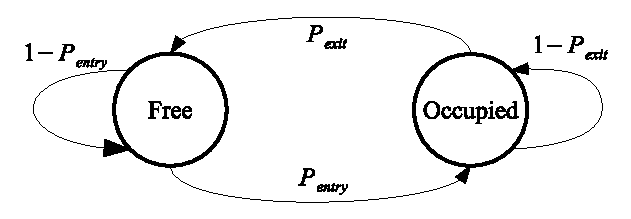
\includegraphics[width=0.7\linewidth]{chapters/mapping_of_dynamic_areas/figures/markow_occupancy_model}
	\caption{Markow chain for occupancy states borrowed from \cite{Saarinen2012}}
	\label{fig:markow_occupancy_model}
\end{figure}

The transitions is modeled as Poisson processes and the rate parameters is estimated as Gamma distributions. This gives in total four variables for each cell, which are used to interpret the type of dynamic for the cell. 

Another method for learning the map dynamics using Hidden Markov Models (HMM) is described by Meyer-Delius et al. \cite{Meyer-Delius2012}. This method uses the same possible states as the IMAC, but as it is a HMM the states are not directly observable thus it is possible to incorporate sensor uncertainty. In order to learn the parameters of the model two methods are used; an offline and an online approach. The offline approach requires storing all observations and then iteratively learn the parameters using the expectation-maximization algorithm. The online version of the parameter learning algorithm, developed by Mongillo and Deneve \cite{Mongillo2008} eliminates the need for storing the whole observation set. Instead only 16 values has to be stored for each cell and the iterative learning can be done online. The online method is capable of handling changing dynamics by using a forget factor. 

A different approach to mapping the dynamics is the Frequency Map Enhancement (FREMEN) proposed by Krajník et al. \cite{Krajnik2014}. This method models the dynamics of each cell by its primary frequency components. 
For prediction of future state the frequencies are reconstructed to a signal, which determines the predicted cell value. 
These uses a limited and constant number of parameters per cell. However, the method also requires the storage of time spans where the prediction went wrong in order to determine when a new model is needed. This significantly increases the memory requirements of the method.

With the reconstructed signal it is possible to predict infinitely long out in the future if it object moves with that frequency. 
This is not the case for Markow processes where the predicted probability for being in a state stabilizes on a constant, after many state changes.
There are also disadvantages with the method.
The most prominent comes from the fact, that it is impossible to recover a signal with a frequency lower than the Rayleigh-frequency of $1/T$, where $T$ is the period. 
This demands for storing measurements for the time period in which objects appears, disappears and appears again. This period can everything from hours for vehicles to days or weeks for stocked product parts. 
It might be possible to degrease the amount of stored information by only storing the average taken over periods, but then it is impossible reconstruct objects moving faster than the period which the average is taken. 

The characteristics of the six methods to improve occupancy grid mapping by learning the dynamics of the environment are outlined in table \ref{tab:learners_characteristics}.

\begin{table}[htbp]
    \centering
    \caption{Characteristics of methods to learn dynamics in occupancy grids.}
    \label{tab:learners_characteristics}
    \begin{tabular}{p{2.6cm} | p{1.6cm} | p{4.cm} | p{2.6cm} | p{1.6cm}}
        \toprule
        \textbf{Name} & \textbf{Memory} & \textbf{Dynamic representation} & \textbf{Learning method} & \textbf{Handles dynamics} \\
        \rowcolor[gray]{0.925}
        TOG & High & Time averaged OG & Online batch & Yes \\
        TSM & High & Time  averaged OG & Random sample replacement  & Yes\\
        \rowcolor[gray]{0.925}
        IMAC & Low & Markov parameters & Online iterative & Yes \\
        HMM - Offline & High & Markov parameters & Offline batch  & No \\
        \rowcolor[gray]{0.925} 
        HMM - Online & Low & Markov parameters & Online iterative & Yes \\
        FREMEN & Medium & Frequency components & Online batch & Yes\\
        \bottomrule
    \end{tabular}
\end{table}

\subsection{Methods ability to learn Markow Processes}
The described methods that models dynamic with Markow processes are compared with a simple simulation where a grid cell are occupied by a dynamic obstacle. 
Whether the cell is occupied or free is controlled by a Markow process with $0.9$ probability for entering and $0.2$ probability for exiting the cell. 
The process is observed by an one dimensional range sensor, which can measure too short with a probability of $0.16$, in which case the online-HMM are propagated one step without adding new information and the IMAC is left unchanged.
There is an equal probability for the sensor measuring a range too far, which results in a reading of an empty cell independently of the cell's state. 
Figure \ref{fig:markow_learning} shows that IMAC is unable to converge to the correct state transition probabilities, where as the HMM-online method that incorporate the uncertainties in measurements slowly converges toward them.
The state transitions estimated by IMAC are so far from the actual parameters that they are almost useless for prediction. 
The number of measurements needed for HMM-online to converge is however very large.
Considering that the simulation is setup so that the object has a considerable possibility of moving between each measurement, it will be very time consuming to learn the transition probabilities for obstacles moving at days between.

\begin{figure}[htbp]
    \centering
    \begin{subfigure}[t]{0.45\textwidth}
        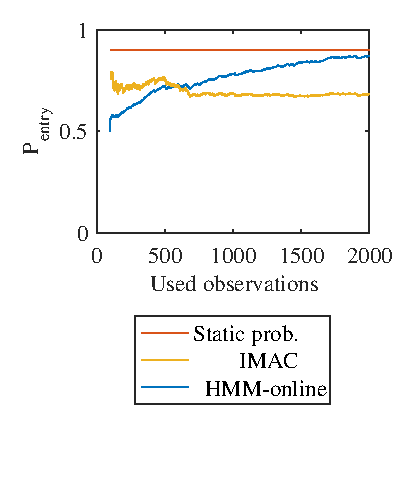
\includegraphics[width=1.0\textwidth]{chapters/mapping_of_dynamic_areas/figures/markow_learn_1d_entry}	
        %\caption{}
        %\label{fig:markow_learn_1d_entry}
    \end{subfigure}
    \begin{subfigure}[t]{0.45\textwidth}
        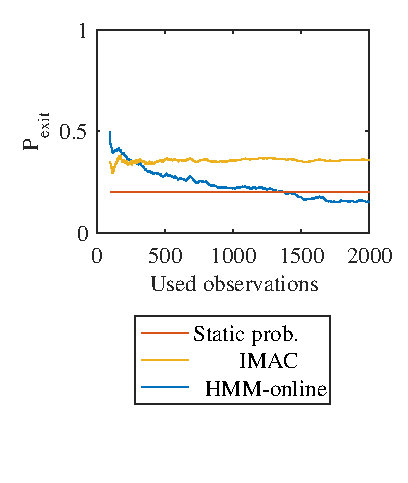
\includegraphics[width=1.0\textwidth]{chapters/mapping_of_dynamic_areas/figures/markow_learn_1d_exit}
        %\caption{}
        %\label{fig:markow_learn_1d_exit}
    \end{subfigure}
    \caption{Learned state transition probabilities compared to the simulated Markow process.}
    \label{fig:markow_learning}
\end{figure}
